\documentclass[11pt,letterpaper,english]{article}
%\documentclass[preprint,review,12pt]{elsarticle}
% Page design
\usepackage[top=1in, bottom=2in, left=1in, right=1in] {geometry}
\usepackage{fancyhdr}
\usepackage{setspace}
\usepackage{lastpage}
\pagestyle{fancy}
\fancyhf{}
\rfoot{\center Page \thepage \hspace{1pt} of \pageref{LastPage}}

% General packages
\usepackage[T1]{fontenc}
\usepackage[utf8]{inputenc}
%\usepackage{txfonts}
\usepackage{xcolor}
\usepackage{soul}
%\usepackage{eqnarray}
\usepackage{epsfig}
\usepackage{epstopdf}
\usepackage{graphicx}
\usepackage{mathptmx}
\usepackage{enumitem}
\usepackage{booktabs}
\usepackage{setspace}
\newcommand{\verbatimfont}[1]{\renewcommand{\verbatim@font}{\ttfamily#1}}
\usepackage{graphicx}
\usepackage{epstopdf}
\usepackage{color}
\usepackage{multirow}
\usepackage{floatrow}
\usepackage{bm}
\usepackage{amsmath}
\usepackage{hhline}
\setlength\doublerulesep{.7pt}
%\usepackage{tabularx}
\usepackage{subcaption}

\usepackage{dsfont}

% Section format
\usepackage{sectsty}
\sectionfont{\normalsize}
\subsectionfont{\normalsize}
\subsubsectionfont{\normalsize \it}
\usepackage{titlesec}
\setlength{\parskip}{\baselineskip}
\setlength{\parindent}{0pt}
\renewcommand{\baselinestretch}{2}

\titlespacing\section{0pt}{0\parskip}{0\parskip}
\titlespacing\subsection{0pt}{0\parskip}{0\parskip}
\titlespacing\subsubsection{0pt}{0\parskip}{0\parskip}
\titleformat{\section}[block]{\normalfont\normalsize\bfseries}{\thesection .}{1em}{}
\titleformat{\subsection}[block]{\normalfont\normalsize\bfseries}{\thesubsection .}{1em}{}
\titleformat{\subsubsection}[block]{\normalfont\normalsize\bfseries}{\thesubsubsection .}{1em}{}

% Bibliography format
\usepackage[hidelinks]{hyperref}
\usepackage{natbib}
\bibliographystyle{humannat}
\usepackage{doi}
\renewcommand{\refname}{REFERENCES}
\makeatletter
%\renewcommand\@biblabel[1]{#1.\em}
\makeatother
\setlength{\bibsep}{0pt plus 0.3ex}

% Captions
\usepackage{caption}
\captionsetup[figure]{labelfont={bf,normalsize},textfont={bf,normalsize},labelformat={default},labelsep=period,name={Figure}}

% Tables
\floatsetup[table]{capposition=top}
\captionsetup[table]{labelfont={bf,normalsize},textfont={bf,normalsize},labelformat={default},labelsep=period,name={Table}}
\renewcommand{\thetable}{\Roman{table}}
\captionsetup[sub]{font={normalsize},labelfont={bf,normalsize}}

% UDF
\definecolor{brown}{RGB}{74,68,42}
\newcommand{\tw}[1]{#1\textwidth}
\newcommand{\lw}{\linewidth}
\renewcommand{\eqref}[1]{(\ref{#1})}

% Turning off highlighting
%\renewcommand{\hl}[1]{#1}

\begin{document}

\vspace*{-0.45in}
\begin{center}
{\Large\centering\bf CFD Evaluation of Pressure Change along Coolant Passages in Sodium-cooled Fast Reactor using Nek5000}

\vspace{3pt}

\begin{spacing}{1}
{\bf \large Jun Fang, Yiqi Yu, Haomin Yuan, Elia Merzari$^\dagger$, Dillon R. Shaver} \\
\large \textit{Argonne National Laboratory, Lemont, IL 60439, USA} \\
\large \textit{$^\dagger$Pennsylvania State University, State College, PA 16801, USA} \\
{\color{brown} fangj@anl.gov (J. Fang), dshaver@anl.gov (D. Shaver)}
\end{spacing}
\vspace{10pt}

\end{center}

\normalsize

\section*{ABSTRACT}

To support the design of advanced Sodium-cooled Fast Reactor (SFR), a series of computational fluid dynamic (CFD) simulations are performed to investigate the pressure change along various flow passages in the proposed SFR system. The simulations are carried out with the state-of-the-art spectral element flow solver, Nek5000. Two specific case studies are presented in this paper: the flow exiting the axial neutron reflector channels and the flow entering the fuel pin bundle. Due to the high Reynolds numbers expected, RANS methods are necessary. A newly developed regularized $k-\omega$ RANS model is adopted in the related CFD calculations. The first case study explores the effect of Reynolds number on the pressure change when flow exiting the reflector channels. The pressure change in this case has two major contributors: the change due to wall friction and the Bernoulli effect. It is found out that the non-dimensional pressure change (i.e. pressure loss coefficient) reduces slightly as the Reynolds number increases. In the second case study, the advanced NekNek coupling capability is tested where an integral domain can be divided into multiple subdomains with an overlapping interface for flow information communication. The preliminary results obtained so far confirmed the consistency between the NekNek results and those produced by regular Nek5000 simulation. The presented work is part of the broader effort to apply cutting-edge CFD techniques in addressing the advanced nuclear reactor design challenges.


\begin{flushleft}
{\bf KEYWORDS} \\
 CFD, Nek5000, Pressure Change, Sodium-cooled Fast Reactor
\end{flushleft}

\section{INTRODUCTION}

Nuclear energy is the most reliable emission-free energy source currently available. To continue harnessing the benefits of nuclear energy and modernize its essential nuclear energy research and development infrastructure, the U.S. Department of Energy (DOE) has launched various programs to stimulate the development of advanced reactor technologies. Among many advanced reactor concepts, the sodium-cooled fast reactor (SFR) stands out with a high fuel efficiency and low output of long half-life radioactive nuclear wastes~\citep{Shaver2019a}. Its design will rely on well-tested, verified, and validated methods as well as leveraging advanced high-fidelity simulation capabilities to bridge existing gaps or to reduce uncertainties~\citep{Shaver2019b}. 

In this paper, computational fluid dynamics (CFD) is employed to perform thermal hydraulic assessment for various flow passages. Knowing these engineering insights (e.g. friction factor or loss coefficient) in the reactor component is important to ensure adequacy of the primary pumps and properly assess the transient behavior of the reactor. The advanced spectral element CFD code Nek5000 is used for this assessment, which has a long history of applications in nuclear energy research~\citep{Merzari2012,Fick2017,Shaver2019,Yildiz2019,Merzari2019}. Specifically, the pressure change is investigated herein. Two specific case studies are presented in this paper: the flow exiting the axial neutron reflector channels and the flow entering the fuel pin bundle. Due to the high density of liquid sodium and the flow rates required to provide adequate cooling to any reactor, the Reynolds numbers anticipated are quite large ($10^6$). It is therefore necessary to use a RANS approach to model turbulence as the computational expense associated with resolving the turbulent fluctuations in a high-fidelity model would be prohibitively large. A newly developed regularized $k-\omega$ RANS model is adopted in the related Nek5000 calculations. The first case study explores the effect of Reynolds number on the pressure change when flow exiting the reflector channels. The pressure change in this case has two major contributors: the change due to wall friction and Bernoulli effect. The non-dimensional pressure change is found out to reduce slightly as the Reynolds number increases. The second case study tested the NekNek coupling capability where the pressure change over an integral domain is compared with that from two separate subdomains. The subdomains are coupled at the overlapped interface. The preliminary results obtained so far have confirmed the consistency between the integral domain results simulated by regular Nek5000 framework and the subdomain simulations coupled by NekNek. The rest of the paper is structured as follows: section 2 introduces the numerical methods used in this work; section 3 will focus on the two separate case studies and show how the state-of-the-art CFD can help in studying the related engineering flow problems; the concluding remarks as well as the future work needed are discussed in section 0. 


%%---------------------------------------------------------------------------%%

%%---------------------------------------------------------------------------%%
\section{Numerical Methods}
\label{sec:nekrs}

Nek5000 is an open source CFD code based on the spectral element method (SEM)~\citep{Patera1984} with a long history of use in reactor thermal-hydraulics research~\citep{Merzari2019a}. SEM combines the accuracy of spectral methods with the domain flexibility of the finite element method. In Nek5000 calculations, the domain is discretized into E curvilinear hexahedral elements, in which the solution is represented as a tensor product of Nth-order Lagrange polynomials based on the Gauss-Lobatto-Legendre (GLL) nodal points, leading to a total number of grid points n=EN3. Nek5000 was designed from the outset of distributed-memory platforms. It is highly parallel and has been previously applied to a wide range of problems to gain unprecedented insight into the physics of turbulence in complex flows~\citep{Merzari2019,Martinez2019}. The time-stepping scheme of Nek5000 is semi-implicit: the diffusion terms of the Navier-Stocks equations are treated implicitly by using a kth-order backward difference formula (BDFk), while nonlinear terms are approximated by a kth-order extrapolation (EXTk)~\citep{Ho1989}. Nek5000 was originally developed for simulating turbulent flows with very high fidelity, i.e. DNS and LES. More recently, the RANS capability has been implemented in the form of the regularized versions of the $k-\omega$ class of models~\citep{Tomboulides2018}. Both LES and DNS require proper resolution of turbulent length scales, which can be very expensive computationally. By using a RANS model, a reasonable balance of computational cost and accuracy is achieved for the flow problems encountered in SFR designs. 

\subsection{Governing equations}
\label{sec:nek1}
For incompressible flow with RANS turbulence model, the Navier-Stokes equations are given by:

\begin{equation}
    \frac{\partial u_i}{\partial x_i}  =  0
\end{equation}

\begin{equation}
 \rho \left[ \frac{\partial u_i}{\partial t} + \frac{\partial }{\partial x_j}(u_i u_j) \right] =  -\frac{\partial p}{\partial x_i} + \frac{\partial }{\partial x_j}\left[(\mu + \mu_t)( \frac{\partial u_i}{\partial x_j} + \frac{\partial u_j}{\partial x_i})\right] + F_i
\end{equation}

where the turbulent viscosity $\mu_t$ is calculated from the turbulent scalars based on the $k-\omega$ model. 
 
The formulation used for this work solved the dimensionless forms of the RANS equations. To simulate fluid flow in Nek5000, the fluid properties must be given, such as fluid density, dynamic viscosity. For an incompressible flow model, these properties are assumed to be constant and only dimensionless groups are necessary as input to the code. These include a non-dimensional density of 1 and the Reynolds number given by

\begin{equation}
    Re = \frac{\rho U_0 D_h}{\mu}
\end{equation}

Additionally, the geometry must be defined on a computational mesh which includes proper boundary conditions, such as inlet, outlet, and wall boundaries. The meshing tool, ICEM-CFD, is utilized here to produce the computational meshes using a blocking strategy. Nek5000 requires the use of hexahedral elements for the computation, but supports the conversion meshes containing tetrahedral and prismatic elements through a custom tet-to-hex converter~\citep{Yuan2020}. Each hexahedral element can be further discretized at run-time using the GLL quadrature based on the selected polynomial approximation order. This allows mesh convergence to be performed by increasing the polynomial order, which is also known as p-type refinement. This strategy is used to ensure the results presented are mesh independent. 

\subsection{The regularized $\lowercase{k}-\omega$ RANS model}
\label{sec:nek2}

The $k-\omega$ model is among the most commonly used RANS turbulence models, which is known to offer better performance for boundary layer, free shear flows compared to other alternatives like $k-\epsilon$ class of models. However, a main drawback associated is the wall boundary condition for $\omega$. According to asymptotic estimates, the value of $\omega$ in the standard $k-\omega$ model becomes infinite at solid walls. The typical treatment is to specify the value of $\omega$ to some large value at grid points on the walls. Although this approach may increase stability, it causes the numerical solution to be sensitive to near-wall grid spacing~\citep{Wilcox1998}. The inability of this approach to provide a grid-independent result aside, such treatment can be problematic in high-order approaches. For the spectral-element method used here, derivative operators are not local in character and assigning an arbitrarily large value at the wall can lead to numerical oscillations. In response, a novel regularized version of the standard $k-\omega$ turbulence model has been recently developed~\citep{Tomboulides2018}. In the regularized formulation, the overall value of $\omega$ is defined as the sum of the value of $\omega$ on the wall ($\omega_W$) and a correction term ($\omega^\prime$). 

\begin{equation}
    \omega = \omega^\prime + \omega_W 
\end{equation}

The singular asymptotic behavior can be then subtracted from the solution. As a result, we can solve for a quantity $\omega^\prime$ that is finite everywhere in the domain. A partial differential equation (PDE) is constructed for the correction term

\begin{equation}
\label{eqn:omega_trans}
\rho \left( \frac{\partial \omega^\prime}{\partial t} + \bf{v} \cdot \bf{\nabla}  \omega^\prime \right) =  \bf{\nabla} \cdot \left[ (\mu+\frac{\mu_t}{\sigma_\omega } ) \bf{\nabla} \omega^\prime \right] + G_{\omega} - Y_{\omega} + S_{\omega_W}
\end{equation}

where $G_{\omega}$, $Y_{\omega}$ and $S_{\omega_W}$ represent the production, the destruction and the extra source terms resulting from the regularization respectively. All source terms in Eq. (\ref{eqn:omega_trans}) are either able to reach a finite limit at walls or cancelled out. Interested readers are referred to~\cite{Tomboulides2018} for a comprehensive discussion of all source terms involved. Meanwhile, it is worthwhile to mention that the derivation of source term $S_{\omega_W}$ assumes a asymptotic relationship of $\omega_W$ near the wall, which is given by 

\begin{equation}
    \omega_W = \frac{a \nu}{\beta_0 y_w^2} 
\end{equation}

where $y_w$ is the distance from the nearest wall and $\beta_0$ is determined from the particular model implementation. The asymptotically correct value of the constant a in the expression above is 6 according to~\cite{Wilcox1998}. Through regularizing the turbulence dissipation frequency in this manner, the transport equation has the convenient Dirichlet wall-boundary condition of $\omega^\prime = 0$, in contrast to the grid-dependent boundary conditions recommended for the non-regularized formulations. This is particularly useful for wall-resolved variants of the $k-\omega$ model and allows the regularized implementation to achieve spectral convergence for increasing mesh resolution. 

The regularized formulation for omega is used with a standard formulation for the turbulent kinetic energy transport equation~\citep{Wilcox1988}

\begin{equation}
\label{eqn:k_trans}
\rho \left( \frac{\partial k}{\partial t} + \bf{v} \cdot \bf{\nabla}  k \right) =  \bf{\nabla} \cdot \left[ (\mu+\frac{\mu_t}{\sigma_k } ) \bf{\nabla} k \right] + G_k - Y_k
\end{equation}

The two turbulence scalars are then used to construct the kinematic eddy viscosity

\begin{equation}
	\nu_t = \frac{\mu_t}{\rho} = \frac{k}{\omega}
\end{equation}

The regularized $k-\omega$ model has been demonstrated to produce results consistent with typical, i.e., non-regularized, implementations~\citep{Tomboulides2018}.


\subsection{The NekNek coupling}
\label{sec:nek3}

The ability to decompose a global domain into separate, but overlapping, subdomains greatly eases mesh generation procedures and increases flexibility of modeling flows with complex geometries. An overlapping mesh methodology has been recently developed in Nek5000, which can allow simultaneous simulation sessions to be carried out for different subdomains and the real-time communication of flow information on the overlapping interface~\citep{Merrill2016}. This novel coupling framework is referred herein as NekNek. The spectral accuracy is maintained for spatial discretization due to a spectral interpolation at interface boundaries using solution approximations in an $N^th$-order polynomial space on GLL points. The global high-order (up to a third) temporal accuracy of the flow solver is also maintained with few, or no, iterations using solutions at previous time steps to form explicit extrapolation approximation at the interface. The NekNek coupling capability has been previously verified in some canonical problems, such as the three dimensional fully-developed turbulent pipe flow with other physical and computational experiments. 
%%---------------------------------------------------------------------------%%
\section{Results and Discussions}
\label{sec:discuss}
The pressure change through various reactor components is a crucial parameter to be considered in designing the SFR system.
Due to the novelty of the proposed concept, many of its components do not have readily applicable correlations and the analysis will rely more heavily on the CFD result for accurate pressure change predictions.
To demonstrate how the related design tasks can be supported by the state-of-the-art CFD flow solver, Nek5000, two case studies are to be presented in this work.
The first problem investigates the jet flow exiting the axial neutron reflector channels and mixing within an upper channel.
The objective here is to evaluate the pressure loss during this process given different flow conditions in terms of the Reynolds numbers.
The second case study will focus on the flow entering the fuel bundle.
A simplified 7-pin bundle is first studied before moving on to the realistic 217-pin bundle.
The related geometry is split into two subdomains to test the NekNek coupling capability.
Meanwhile, an integral domain case is also computed as a reference for the NekNek results.
 


\subsection{Case study I: flow exiting the axial neutron reflector}
\label{sec:results1}

The computational domain used in the first case study is illustrated in Figure~\ref{fig:reflector}, which consists of three semi-circular inlet channels inside the reflector and a wider vertical hexagonal channel above the reflector.
The inlet semi-circular channels have a 2.5 cm nominal radius while the full domain height is 18.4 cm.
Both the upper and inlet channels are extruded.
The extrusion of the upper domain helps avoid the recirculation issue at the outlet boundary.
Meanwhile, the elongated inlet allows a fully developed turbulent inflow produced by the recycling velocity boundary condition.
Three Reynolds numbers are considered, including 20,000, 50,000 and 900,000.
Since the non-dimensional calculations are carried out here, the increase of Reynolds number is achieved by decreasing the flow viscosity.

\begin{figure}[!ht]
\centering
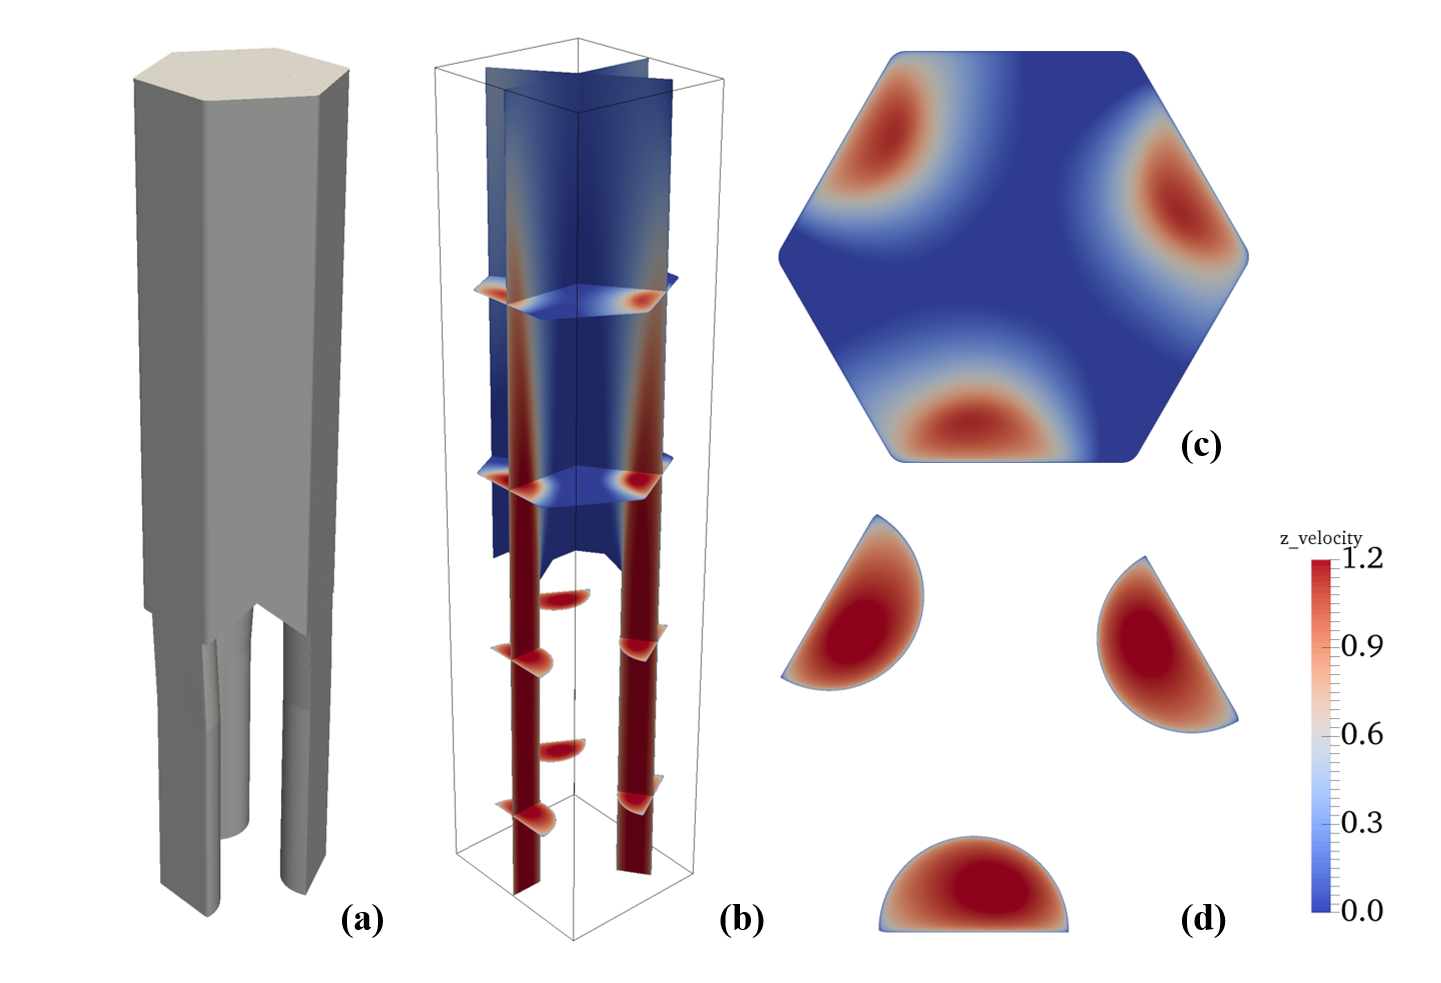
\includegraphics[width=0.8\textwidth]{./figures/reflector_domain.png}
\caption{The computational domain and steady-state velocity fields at Re of 20,000: (a) the side view; (b) the velocity fields on various cut planes; (c) a cut plane at the upper channel; (d) a cut plane over the reflector/inlet legs. }
\label{fig:reflector}
\end{figure}


The distributions of velocity, TKE ($k$) and turbulence dissipation frequency ($\omega$) are presented in Figure~\ref{fig:reflector_vel}, Figure~\ref{fig:reflector_tke}, and Figure~\ref{fig:reflector_omega} respectively.
Overall, the turbulent flow displays similar profiles at the three Reynolds numbers.
Some subtle difference is observed in the velocity profile.
For instance, as shown in Figure~\ref{fig:reflector_vel}, the wake propagates longer with a higher Re.
Also, the flow re-circulation is captured with negative streamwise velocity observed right after the joint region between the reflector channel and the upper channel.
A high TKE region is noticed in the upper channel, of which the shape coincides with that the velocity profile.
It indicates that a strong mixing process is going on when the jet comes out from the reflector into the upper space.
As for the turbulence dissipation frequency, it is noticeably higher in the near wall region as well as where the strong mixing takes place.
Again, all the calculations are done in a non-dimensional manner, and the slightly decrease in maximum TKE in Figure~\ref{fig:reflector_tke} should not be confused as the decrease in the actual TKE for higher Reynolds numbers.
In all simulations, the $y^+$ value is monitored and ideally the closest layer of GLL points should be within $y_p^+ < 1$.
So far, this restriction is only strictly kept in the case with Re of 20K.
Appropriate boundary layer mesh refinement may be needed for high Re cases in the future.

\begin{figure}[!ht]
\centering
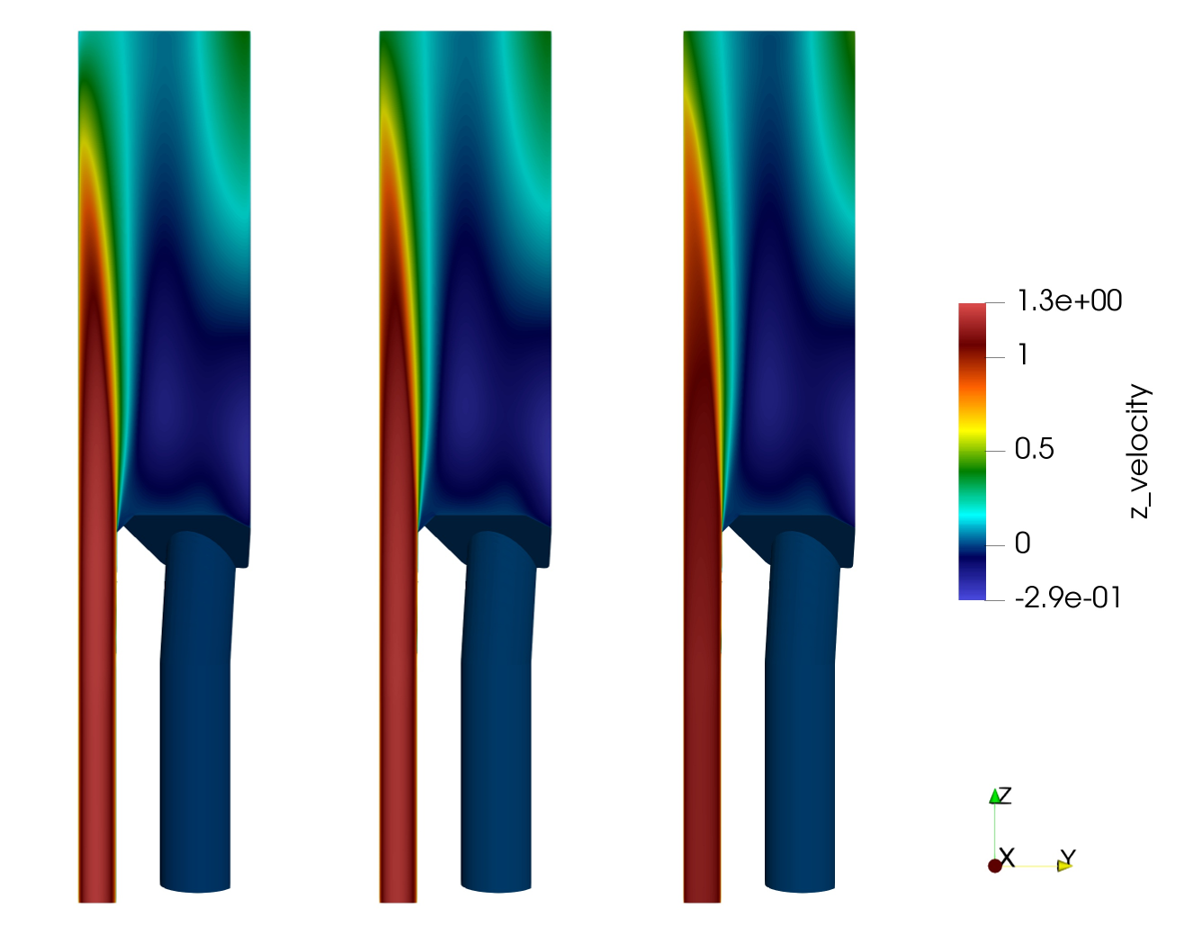
\includegraphics[width=0.8\textwidth]{./figures/reflector_vel.png}
\caption{The steady state streamwise velocity profiles at Re = 20,000, 50,000, 900,000 (from left to right). }
\label{fig:reflector_vel}
\end{figure}

\begin{figure}[!ht]
\centering
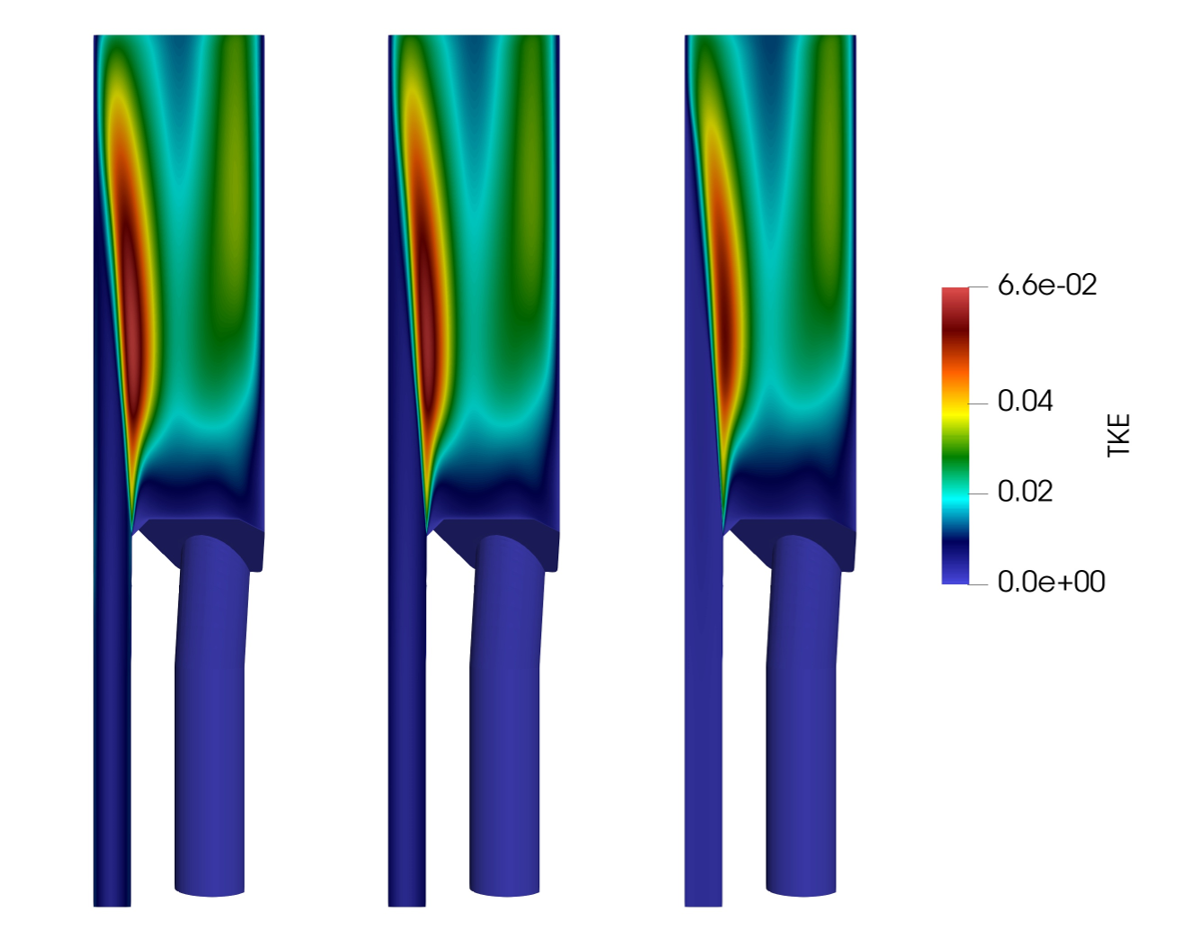
\includegraphics[width=0.8\textwidth]{./figures/reflector_tke.png}
\caption{The steady state turbulent kinetic energy profiles at Re = 20,000, 50,000, 900,000 (from left to right). }
\label{fig:reflector_tke}
\end{figure}

\begin{figure}[!ht]
\centering
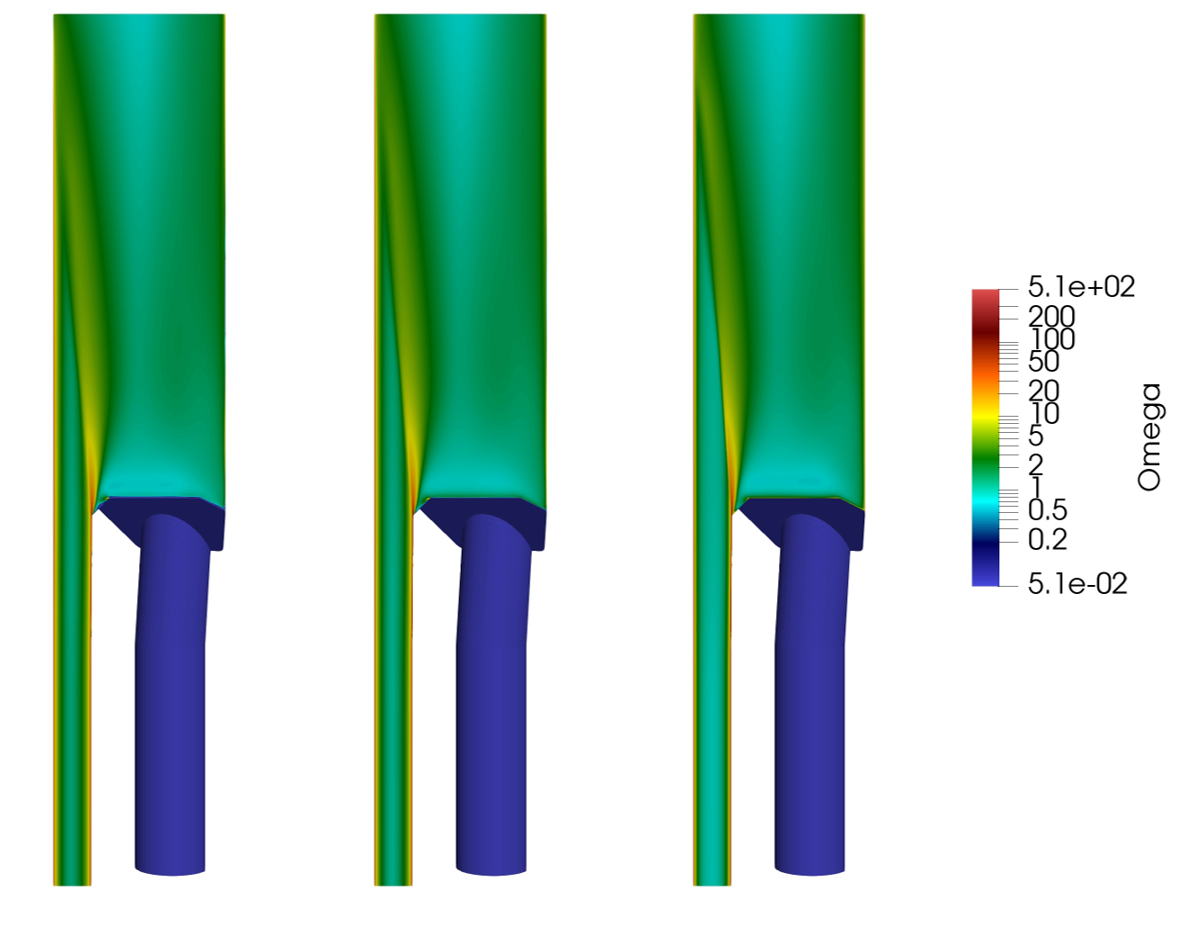
\includegraphics[width=0.8\textwidth]{./figures/reflector_omega.png}
\caption{The steady state turbulence dissipation frequency profiles at Re = 20,000, 50,000, 900,000 (from left to right) with a log scale. }
\label{fig:reflector_omega}
\end{figure}

To quantify the pressure change as the flow moves out of the semi-circular channels into a wider upper channel, the area-averaged flow quantities are first extracted at both the domain inlet and outlet.
For example, the average pressure and streamwise velocity at the inlet are computed as follows: 

\begin{equation}
    P_{in} = \frac{1}{A_{in}} \oint P \cdot dA_{in}
\end{equation}

\begin{equation}
    u_{in} = \frac{1}{A_{in}} \oint u \cdot dA_{in}
\end{equation}

A pressure difference is readily obtained by subtracting the inlet pressure from the outlet pressure (i.e.\ $\Delta P_t = P_{out} - P_{in}$).
The pressure change in the current domain has two important contributors, the wall friction effect and the Bernoulli effect due to the change of channel shape.
For the incompressible flow, the Bernoulli principle can be expressed by the equation below: 

\begin{equation}
    \frac{u_{in}^2}{2} + gz_{in} + \frac{P^\prime_{in}}{\rho} = \frac{u_{out}^2}{2} + gz_{out} + \frac{P^\prime_{out}}{\rho}
\end{equation}


where $P^\prime_{in}$ and $P^\prime_{out}$ are theoretical inlet and outlet pressures if the wall friction is assumed to be zero or the Bernoulli effect is the only contributor of pressure change.
It is straightforward to get Eq.~(\ref{eqn:dpb}) based on the energy conservation.
The mean flow slows down as it moves from the narrow passage of the semi-circular channels into a wider plenum.
The gravitational acceleration ($g$) is zero in all cases, so the pressure change due to Bernoulli effect can be estimated by 

\begin{equation}
\label{eqn:dpb}
    \Delta P_B = P^\prime_{out} - P^\prime_{in} = \frac{\rho ( u_{in}^2 - u_{out}^2 )}{2} 
\end{equation}

In reality, the wall friction would always induce additional pressure loss.
Then the pressure change due to the wall friction is given by 

\begin{equation}
    \Delta P_F =  \Delta P_t -\Delta P_B
\end{equation}

In the current Nek5000 simulations, a constant non-dimensional inlet velocity is utilized in all the cases.
Since the flow is incompressible, the outlet velocity would be identical as well due to the mass conservation.
Thus the non-dimensional pressure changes due to the Bernoulli effect will in turn be the same.
Unlike the pressure change due to the Bernoulli effect, the pressure loss owing to the wall friction shows a log-linear dependency on the Reynolds (as shown in Figure~\ref{fig:pressure_loss}).
The non-dimensional pressure change or pressure loss coefficient drops as the Reynolds number increases.
A more detailed summary of pressure change results is provided by Table I.


\begin{figure}[!ht]
\centering
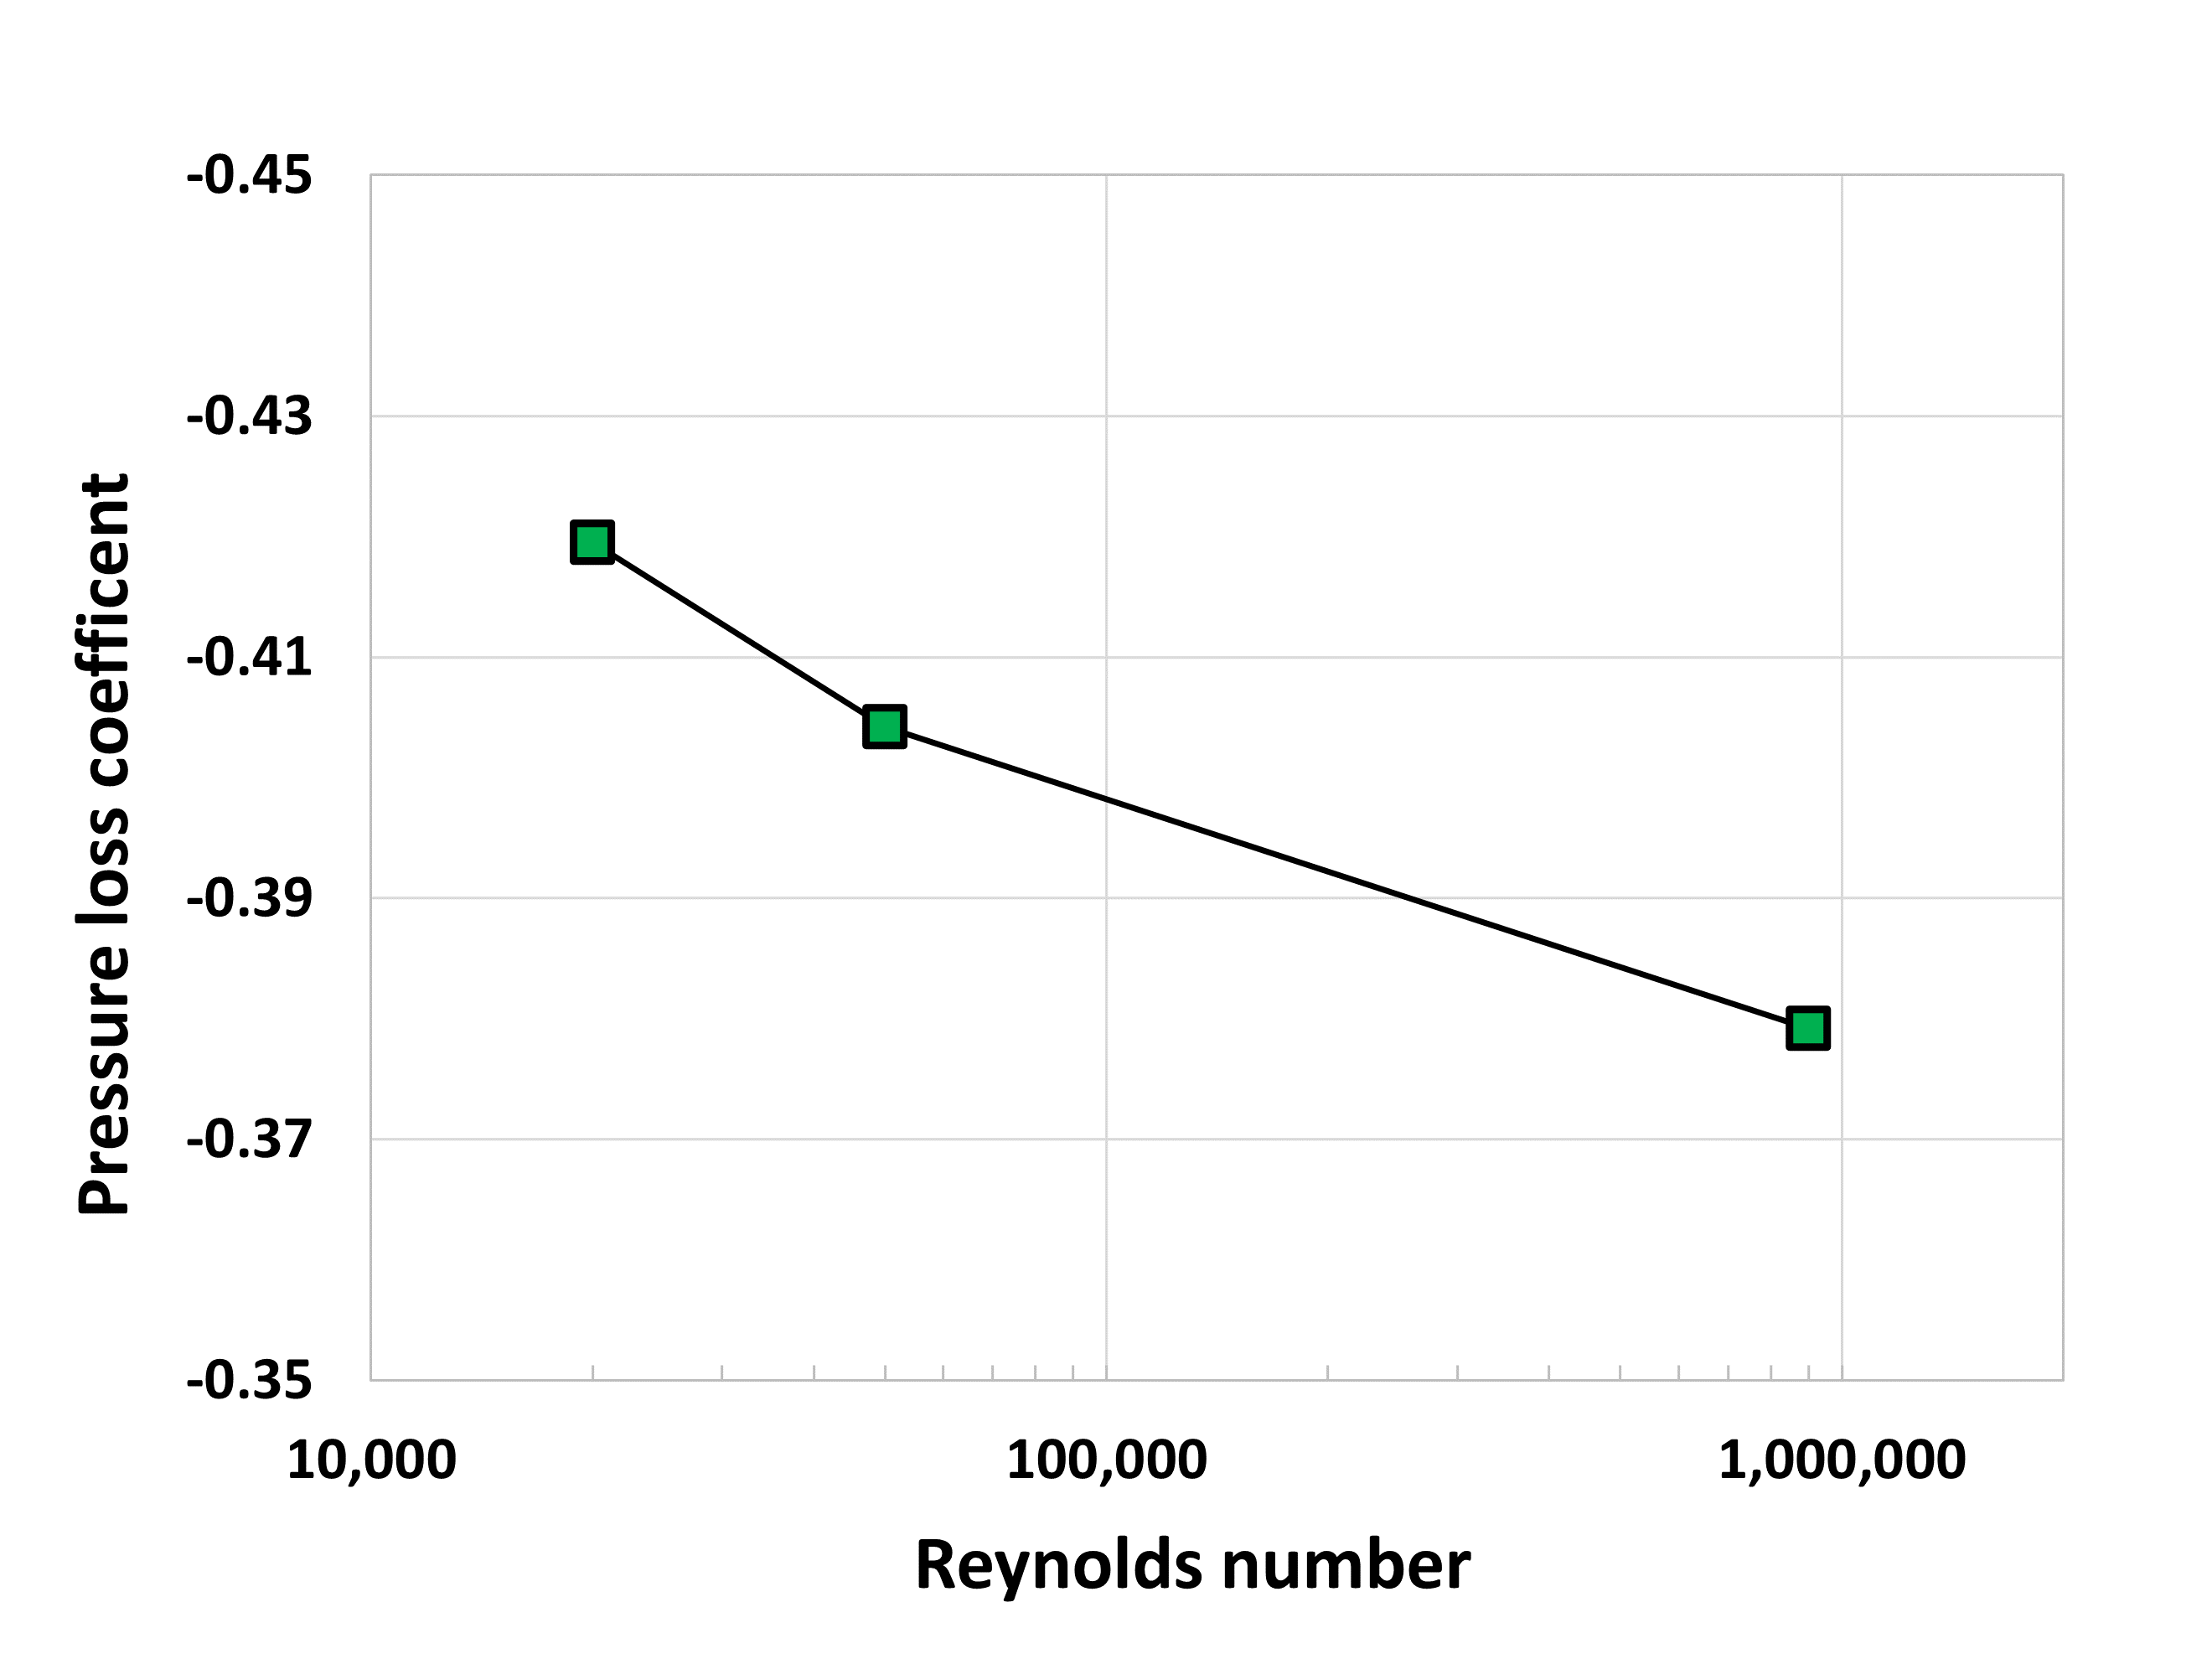
\includegraphics[width=0.6\textwidth]{./figures/pressure_loss.png}
\caption{The pressure loss coefficient due to the wall friction at different Reynolds numbers. }
\label{fig:pressure_loss}
\end{figure}

\begin{table} \centering \small
% \resizebox{0.48\textwidth}{!}{
 \begin{tabular}{ccccc} \hline \hline
   Re        & $\Delta P_t$   & $\Delta P_B$  & $\Delta P_F$  \\ \hline
   20,000    & 4.10E-02       & 2.81E-01      & -4.19E-01  \\
   50,000    & 5.62E-02       & 2.81E-01      & -4.04E-01  \\
   900,000   & 8.13E-02       & 2.81E-01      & -3.79E-01  \\
   \hline \hline
\end{tabular}
 \caption{The summary of pressure changes.}
 \label{tab:full core}
\end{table}



\subsection{Case study II: flow entering the pin bundle}
\label{sec:results2}

The second case study aims to test a novel simulation framework, NekNek, and demonstrate its usefulness in complex engineering geometries.
A two-step approach is employed here: (i) a 2D backward facing step (BFS) case is first simulated to verify the NekNek performance; and (ii) the application of NekNek in simulating the flow entering a 7-pin fuel pin bundle geometry.
The BFS case is selected because of the complex flow physics expected, such as the separation and shear flow.
The BFS domain used in NekNek testing consists of two subchannels: an inlet with a length of 5.5 (0 to 5.5) and an outlet with a length of 20.0 (4.5 to 24.5) as shown in Figure~\ref{fig:bfs_domain}; two subdomains have an overlapped region from 4.5 to 5.5.
The step height is 1.0 and a constant inflow velocity condition is given at the inlet face.
The corresponding Reynolds number is 5,000.
In addition to the NekNek test, a reference case is computed with the regular Nek5000 approach in an integral BFS domain.


\begin{figure}[!ht]
\centering
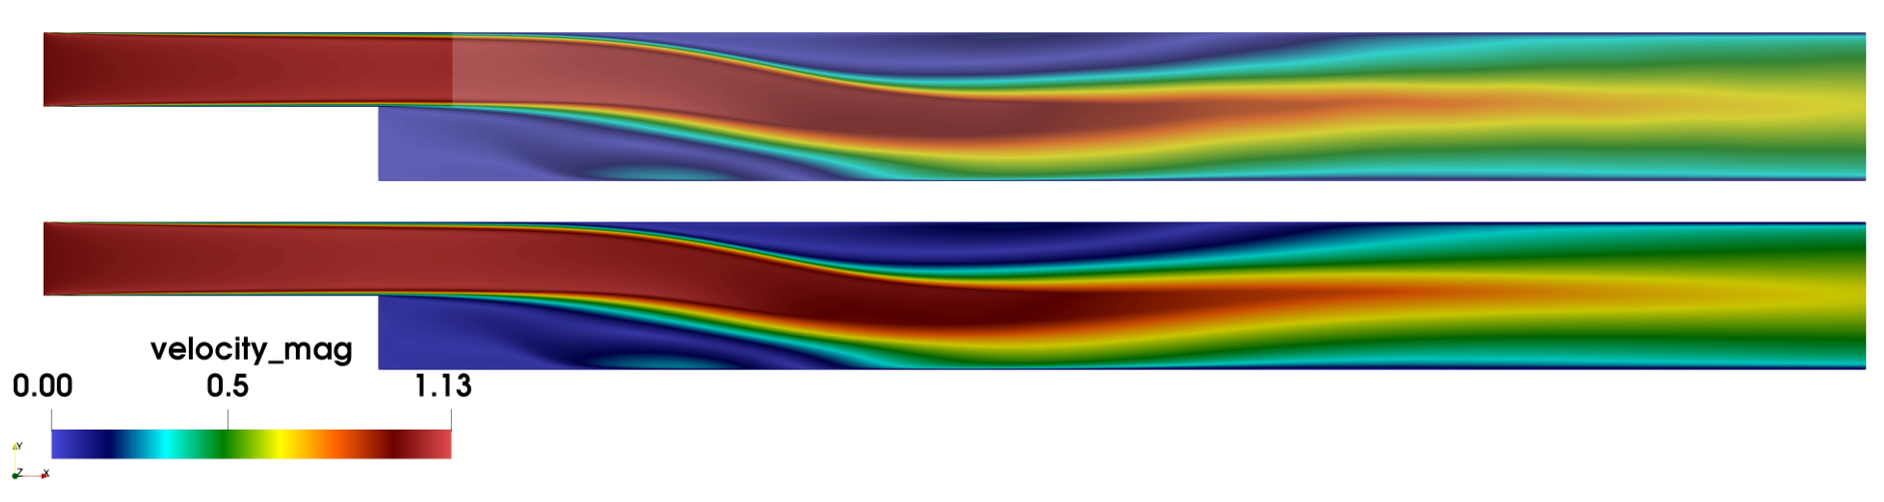
\includegraphics[width=0.9\textwidth]{./figures/bfs_vel.png}
\caption{The steady-state velocity field in decomposed NekNek subdomains (top) and the integral reference domain (bottom). }
\label{fig:bfs_domain}
\end{figure}

It is already qualitatively confirmed in Figure~\ref{fig:bfs_domain} that the NekNek approach can reproduce the overall flow behaviors as compared to those from the integral domain with regular Nek5000 approach.
The boundary layer detachment is observed at the step edge.
A re-circulation zone is created after the step and the flow eventually reattaches at roughly the same downstream location.
A further scrutiny is carried out to compare the local data extracted.
Figure~\ref{fig:bfs_results} compares the streamwise velocity and the turbulent kinetic energy along the line, $y=1.5$, throughout the BFS.
Nearly identical results are produced from the NekNek approach and regular Nek5000 approach, which is a strong indicator of NekNek consistency.
Smooth transition is observed for the quantities of interest over the overlapped region.
It is worthwhile to point out that the continuity of pressure is not kept over subdomains as illustrated in Figure~\ref{fig:bfs_pressure}.
Instead, the pressure gradient is strictly preserved, which is of paramount importance in incompressible flow solver.
If one shifts the original pressure profile in the inlet region (i.e.\ the blue curve) down, it can perfectly match the pressure transition at the corresponding location in the integral domain (represented by the green curve).

\begin{figure}[!ht]
\centering
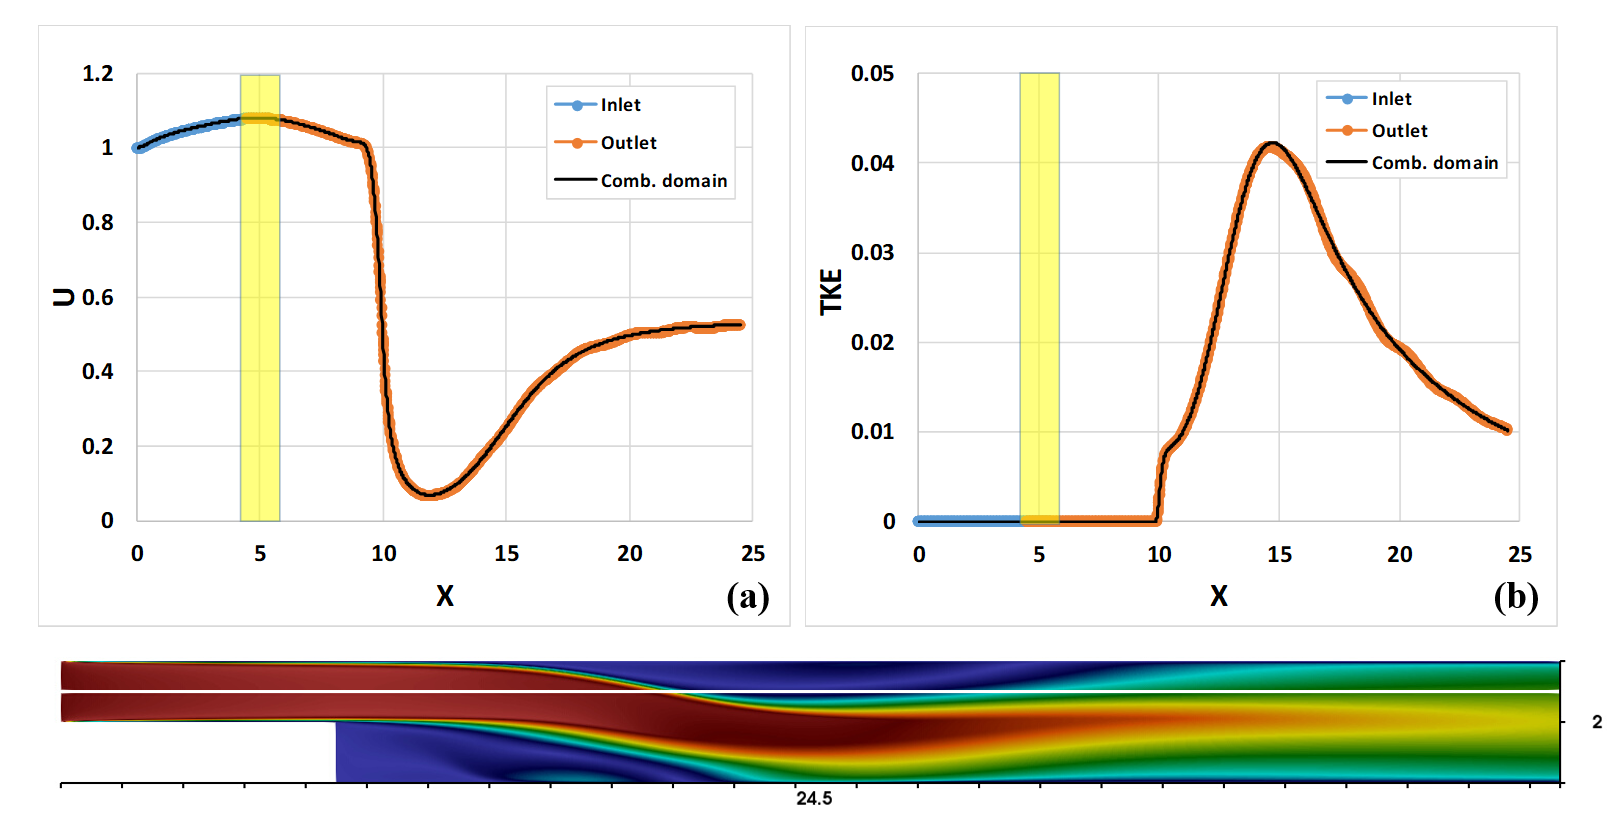
\includegraphics[width=0.8\textwidth]{./figures/bfs_neknek_results.png}
\caption{The steady-state profiles of streamwise velocity (U) and the turbulent kinetic energy (TKE) along the line ($y=1.5$). The yellow band indicates the bounds of overlapped region between subdomains. }
\label{fig:bfs_results}
\end{figure}

\begin{figure}[!ht]
\centering
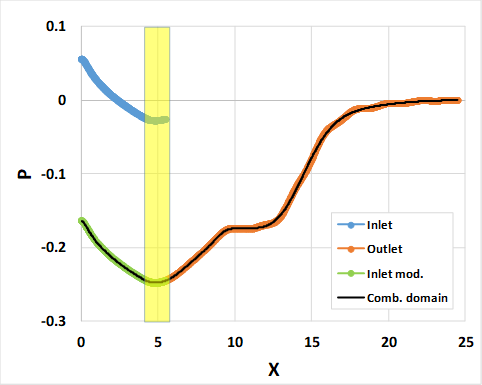
\includegraphics[width=0.6\textwidth]{./figures/bfs_neknek_pressure.png}
\caption{The steady-state pressure distribution along the line ($y=1.5$). }
\label{fig:bfs_pressure}
\end{figure}

As the next step, the NekNek is applied to simulate the flow entering the fuel pin bundle.
A prototypical fuel bundle proposed for the SFR consists of 217 pins, and a simplified 7-pin bundle is considered here.
The 7-pin bundle is adequate for the testing purpose and offers a much shorter turnaround time.
As shown in Figure~\ref{fig:bundle_domain}, the geometry can be divided into two partitions: an upper subdomain contains the pin bundle and supporting structures, and a lower subdomain which is a vertical channel.
The two subdomains overlap at the shared boundary illustrated in Figure~\ref{fig:bundle_domain} by the line between the upper subdomain (in red) and the lower subdomain (in blue).
Two simultaneous simulation sessions are carried out in NekNek coupling for the flow in upper and lower subdomains, and the flow information is exchanged at the overlapping interface.
Meanwhile, the integral domain is also simulated here with the regular Nek5000 approach to serve as the reference.
The primary quantity of interest in this study is the pressure change when flow enters the fuel pin bundle.

\begin{figure}[!ht]
\centering
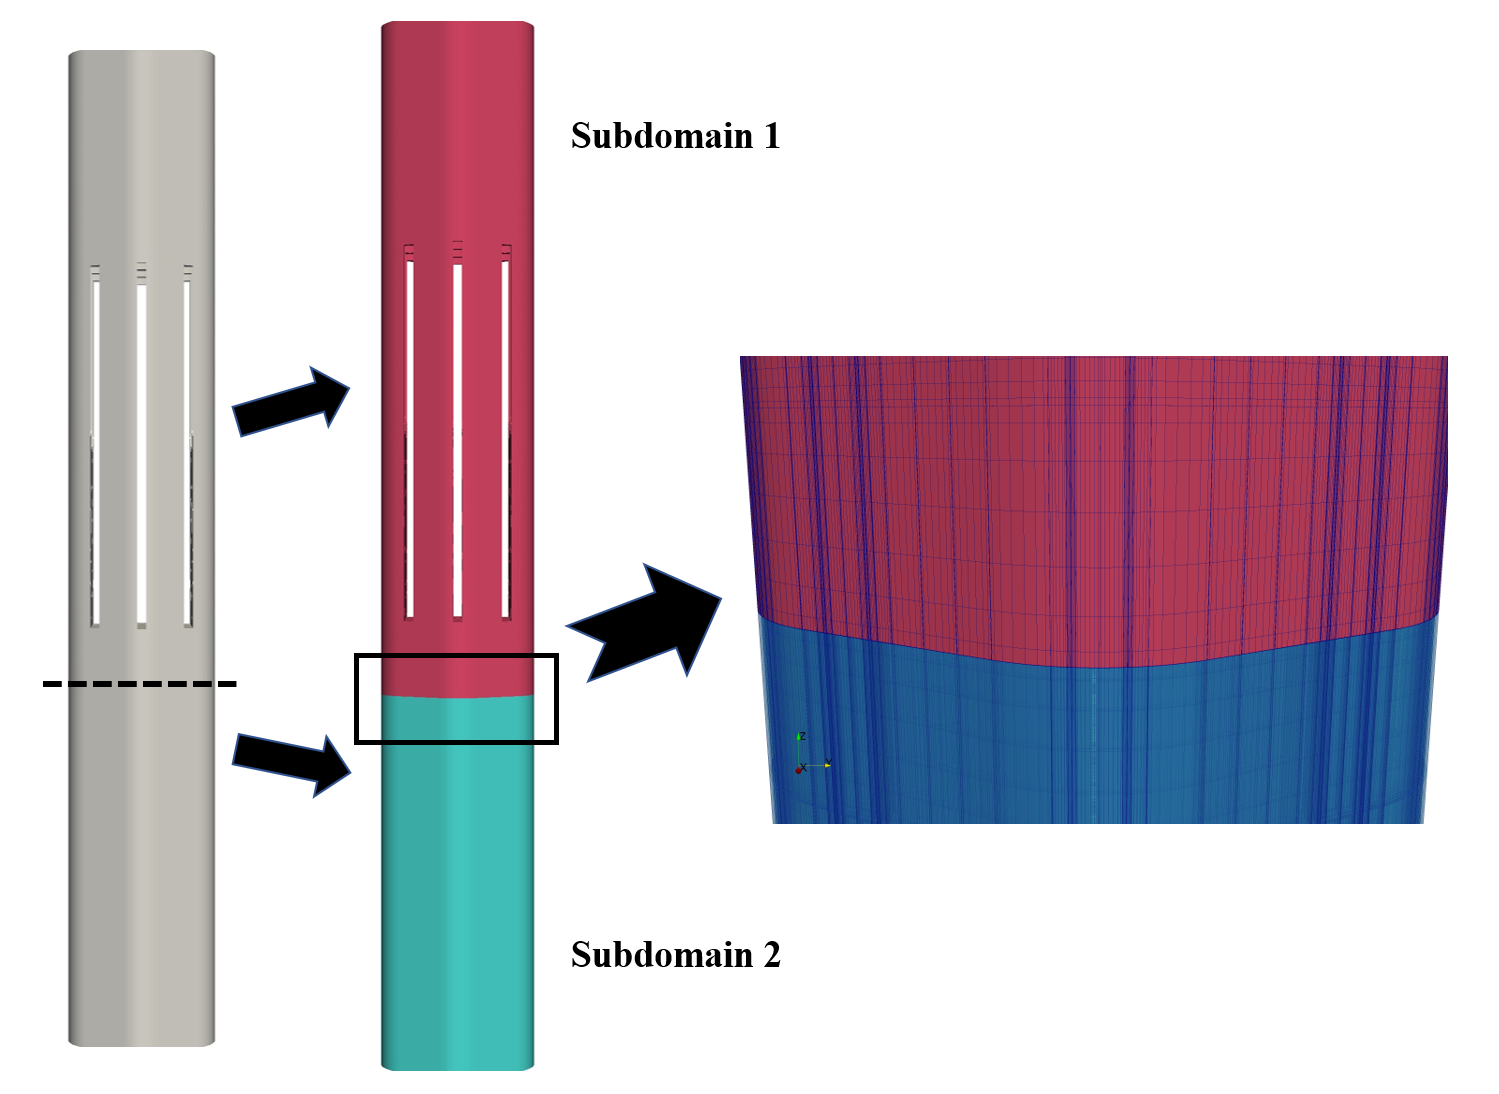
\includegraphics[width=0.8\textwidth]{./figures/bundle_neknek_domain.png}
\caption{The integral domain for the 7-pin demonstration case and the corresponding subdomains utilized in NekNek coupling. }
\label{fig:bundle_domain}
\end{figure}

The quasi-steady-state streamwise velocity distribution is showed in Figure~\ref{fig:bundle_vel}.
The velocity profiles are almost identical except for the slight difference of unsteady wakes induced by supporting structures in the upper domain.
A significant acceleration is observed due to the flow passage narrowing as the flow enters the fuel pin bundle.
Following the same analysis strategy in the case study I, the total pressure change/loss is -9.832 in the integral domain while the pressure changes from two subdomains are -9.734 and -0.117 respectively.
An excellent agreement is obtained again for the pressure data with only a 0.2\% deviation.
Although extended verification efforts may still be needed, the consistency observed here is promising and the related efforts serve as an important stepping stone towards the NekNek application in more realistic/challenging engineering problems.

\begin{figure}[!ht]
\centering
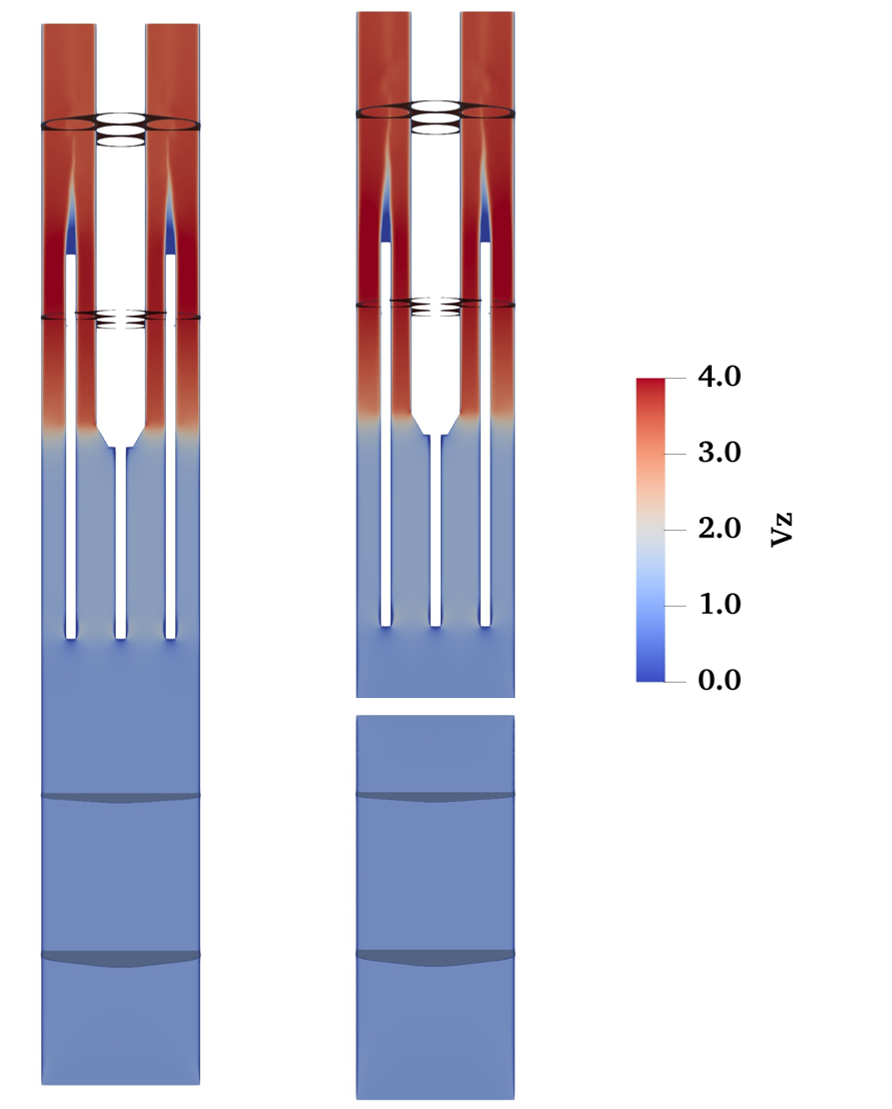
\includegraphics[width=0.5\textwidth]{./figures/bundle_neknek_results.png}
\caption{The quasi-steady-state streamwise velocity from the integral domain (left) and NekNek subdomains (right). }
\label{fig:bundle_vel}
\end{figure}


%%---------------------------------------------------------------------------%%

\section{CONCLUSIONS}

As an important design parameter, the pressure change is investigated for various flow passages in the proposed Sodium-cooled Fast Reactor concept. Two specific case studies are presented in this paper: the flow exiting the axial neutron reflector channels and the flow entering the fuel pin bundle. A newly developed regularized $k-\omega$ RANS model is adopted in related CFD calculations. The first case study explores the effect of Reynolds number on the pressure change. The pressure change in this case has two major contributors: the change due to wall friction and Bernoulli effect. Due to the nature of non-dimensional calculations employed herein, the contribution of Bernoulli effect stays constant at different Reynolds numbers. The non-dimensional pressure change reduces slightly as the Reynolds number increases. The second case study tested the NekNek coupling capability where the pressure change over an integral domain is compared with that from two separate subdomains. The subdomains are coupled at the overlapped interface. The preliminary results obtained so far have confirmed the consistency between the integral domain results simulated by regular Nek5000 framework and the subdomain simulations coupled by NekNek. As a work-in-progress, future investigations are needed. Some examples include i) performing selected high-fidelity simulations (e.g. DNS/LES) at affordable computational expenses to verify the RANS model applicability, ii) the boundary layer mesh improvement in the first case study, and iii) more extensive comparison should be done for the NekNek verification in complex engineering geometries. Nevertheless, it is safe to conclude that the CFD analysis will play an increasingly important role in addressing advanced reactor design challenges. 


\section*{Acknowledgments}

This work was supported by the Nuclear Energy Advanced Modeling and Simulation (NEAMS) program of the U.S. Department of Energy, Office of Nuclear Energy, under contract No. DE-AC02-06CH11357. The authors gratefully acknowledge use of the computing resources provided on Bebop, a high-performance computing cluster operated by the Laboratory Computing Resource Center (LCRC) at Argonne National Laboratory. 


\clearpage
\bibliography{references}

\clearpage
\begin{center}
\scriptsize
\framebox{\parbox{2.6in}{The submitted manuscript has been created by UChicago Argonne, LLC, Operator of Argonne National Laboratory
("Argonne").  Argonne, a U.S. Department of Energy Office of Science laboratory, is operated under Contract No. DE-AC02-06CH11357.  The U.S. Government retains for itself, and others acting on its behalf, a paid-up, nonexclusive, irrevocable worldwide license in said article to reproduce, prepare derivative works, distribute copies to the public, and perform publicly and display publicly, by or on behalf of the Government.}}
\normalsize
\end{center}


\end{document}
